\subsubsection{Design of Registers} \label{sec:design-registers}

As discussed in Section \ref{sec:design-instruction-set}, in ZKVM, we must not only constrain the state of the registers associated with the instruction being updated correctly, 
but we must also ensure that the state of the registers not involved in the current instruction remains unchanged. 
While register-based VMs offer certain advantages, having a larger number of registers is not necessarily better from a verification standpoint. 
There is a trade-off that must be considered:
\begin{itemize}
    \item How many registers will be sufficient for most of the calculations?
    \item For some calculations, is the increased number of memory accesses acceptable when there are not enough registers?
\end{itemize}

If the number of registers is small enough and memory accesses don't need to be constrained, this would be the ideal scenario for verification efficiency. 
The design of the \href{https://starkware.co/cairo/}{Cairo VM} exemplifies this approach, with no general-purpose registers and all instruction operands originating from memory. 
To avoid consistency checks on memory, a write-once model is employed, meaning memory can't be rewritten at the execution level, obviating the need for checks.

However, the write-once model's downside is that it's unfriendly to Dapp developers, and the memory model's limitations require developers to be extra mindful of memory usage. 
The traditional memory model is the read-write model.

\begin{figure}[!ht]
    \centering
    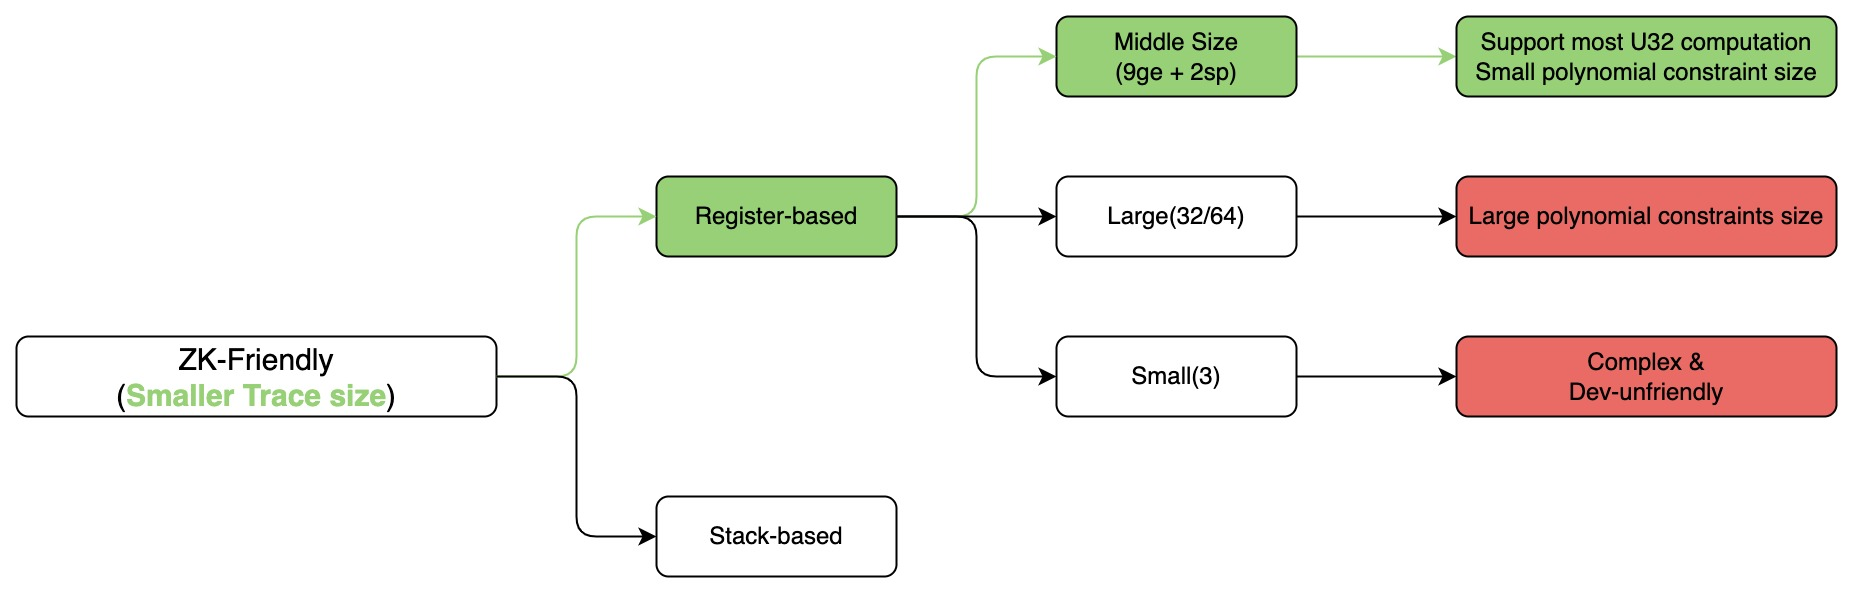
\includegraphics[width=0.6\textwidth]{vm/design-zk-friendly-register.jpeg}
    \caption{How to get ZK-Friendly(Smaller Trace) from register}
    \label{fig:design-zk-friendly-register}
\end{figure}

As illustrated in Figure \ref{fig:design-zk-friendly-register}, we have opted for an optimal solution that takes into account both ZK-Friendly and Dev-Friendly perspectives. 
When it comes to the number of registers, we have considered the fact that the minimum type of computation that can be supported on OlaVM is U32 integer computation. 
With some boundary conditions such as the number of loops, loop termination conditions, etc., we have determined that nine general-purpose registers can support most of the U32 computation. 
Furthermore, both U64 and U256 integer computations can be implemented through the U32 library. 
OlaVM utilizes two special registers (PC and PSP) as well, as explained in Section \ref{subsec: instructions-set}.

If the number of registers is insufficient, we need to use memory for caching, which necessitates memory access-related instructions (MLOAD, MSTORE). 
It is important to note that in order to facilitate FFT, Provers often add redundant data in Trace to meet the size of Trace to the power of 2. 
These redundant data can be replaced with valid data, as demonstrated in Figure \ref{fig:design-better-trace-layout}.

\begin{figure}[!ht]
    \centering
    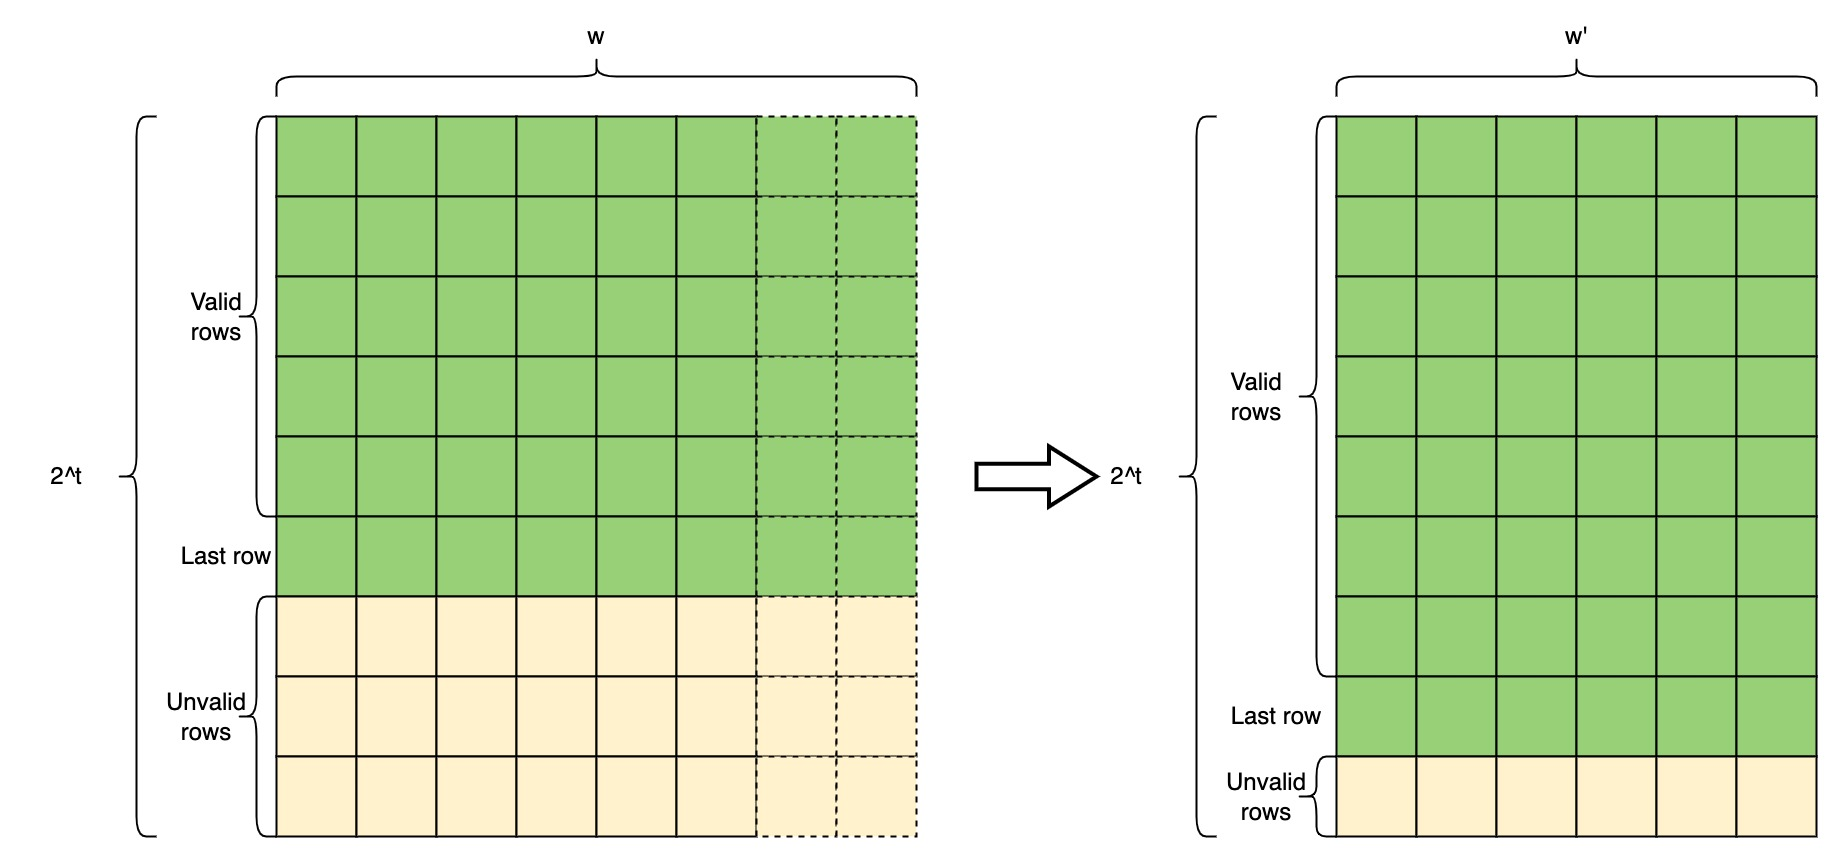
\includegraphics[width=0.6\textwidth]{vm/design-better-trace-layout.jpeg}
    \caption{Better layout of Trace}
    \label{fig:design-better-trace-layout}
\end{figure}
